\chapter{Convolution in Convolution for Network in Network}

{\small \textbf{Authors}\\
Yanwei Pang, \textit{Senior Member, IEEE}, Manli Sun, Xiaoheng Jiang, and Xuelong Li, \textit{Fellow, IEEE}\\ \\
IEEE TRANSACTIONS ON NEURAL NETWORKS AND LEARNING SYSTEMS\\VOL. 29, NO. 5, MAY 2018}

\section{Proposed Method}

In the following paper we are going to talk about another type of CNN. The proposed method comes from another architecture called \textit{Network in Network} (NiN). The main difference between a NiN and a conventional CNN is that the linear filter is replaced by a \textit{multilayer perceptron} (MLP). As a MLP is a nonlinear activation function and we are replacing a filter that is linear, we can consider the MLP as a small network. Another evident difference is that by employing MLP we end up having a very dense connected structure, while previously with filters, we had a shared approach.\\ \\
The proposed method here is called \textit{Convolution in Convolution} (CiC) and is an improved version of NiN. In CiC, an unshared convolution is applied on the \textit{depth} (that is like applying a sparsification on connections), while a shared convolution is applied on the spatial domain (\textit{$width \times height$}). As it turned out from other papers, sparsifying is a good idea when we want to reduce both the overfitting and the number of the parameters as well as it has done here. As regards the difference between a NiN and the proposed CiC, we have that in a CiC, the MLPs (that are used as filters in NiNs) are divided into two categories: \textit{fully sparse MLP} and \textit{partially sparse MLP}. In order to have a more precise idea of what they are, we show their representation in Figure \ref{fig:07_1}. It turns out that the best configuration is the MLP-dense-sparse-dense because it is not possible to have sparsification in the first layer. Moreover, for the sake of the clarity, in the shown image, '0' means dense (fully-connected) and '1' means sparse.\\

\begin{figure}[h!]
    \centering
    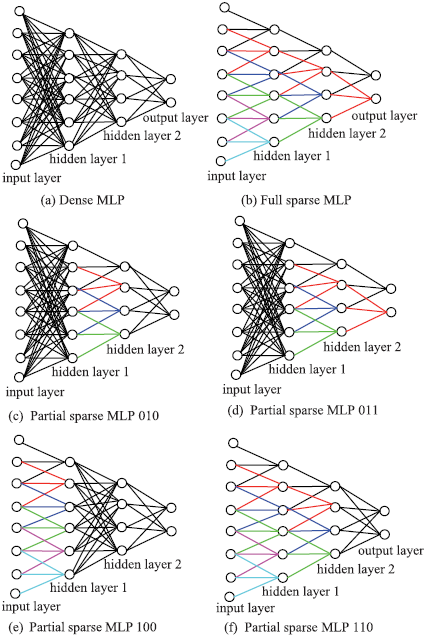
\includegraphics[scale=0.85]{images/07_1.png}
    \caption{(a) Fully connected MLP. (b) Full sparse MLP. (c)–(e) Different types of partial sparse MLPs.}
    \label{fig:07_1}
\end{figure}

\FloatBarrier

\section{Experimental Results}

Experimental results have been evaluated using two structures on different architectures and datasets. Also here data augmentation is performed and in this case we end up having different versions of the original datasets. More specifically, CIFAR10 \citep{CIFAR10and100} and CIFAR100 \citep{CIFAR10and100} become CIFAR10+, CIFAR10++ and CIFAR100+. The two abovementioned structures are respectively: CiC-1-D and CiC-3-D. The difference between them is that in the first one, the convolution (in the spatial domain) is performed with a $1 \times 1$ filter (and in one dimension as regards the depth), while in the second one we increase the size to $n \times n$ and we consider three dimensions filtering. Both structures behave well on the provided datasets, in fact they achieve very good test error rates that validate the following method. 
